\documentclass{article}
\usepackage[utf8]{inputenc}
\usepackage[T1]{fontenc}
\usepackage{graphicx}
\usepackage{hyperref}
\usepackage{geometry}
\geometry{margin=1in}

\title{WILLLAMSBURG}
\date{Encyclopaedia Britannica (1771)}

\begin{document}
\maketitle

\section*{Historical source}
\textbf{Entry ID:} \texttt{entry-willlamsburg-258} \\
\textbf{Volume ID:} 191679021 \\
\textbf{Character Count:} 1170

\subsection*{Extracted Text}
WILLLAMSBURG, e town of North America, in Virginia, and formerly capital of that fact. It is fuated between two rocks; one falling into James, and the other into York River. The distance of each landing place is about a mile from the town, which, with the chief advantage of not being able to bring large wells, and she want of enterprin in the inhabitants, has occhedinal as decay. Here is a college, designed for the education of the Indians, but which, as account of their services to learning, overau-fered the purple. It is 60 miles east of Richmond. W. Long, 76, 30, N. Las 27, 10.

WILLUMSMSTADLY as fees-port town of Holland. It is a handsome frong place, and the harbor is well frequented. It was built by Willimpin price of Oman in 1583 I and in 1733 included to the flashside of Erland. The river near which it is built is called \_Butterliot or Holland Day\_ , and is one of the bulwals of the Dutch on the life of Pakistan, where they always keep a garrition. This place made a gallant defence in 1759 against the French, who were obliged to take the firege. It is 15 miles northcraft of Bergenea-Zoon, and 12 southwell of Dorte. E. Lang, 4-30, N. Las 51, 39.



\section*{Source record}
\begin{itemize}
\item \textbf{Dataset:} \texttt{NationalLibraryOfScotland/encyclopaedia\_britannica\_illustrated}
\item \textbf{Dataset Revision:} \texttt{309f765b1ecc83e0a7f7762e44b4a927a7555443}
\item \textbf{Page ID:} \texttt{britannica:309f765b1ecc83e0a7f7762e44b4a927a7555443:train:258} \\
  \textbf{Filename:} \texttt{page-0258-631a7ae7df34.jpg} \\
  \textbf{Row Index:} 258 \\
  \textbf{SHA256:} \texttt{631a7ae7df340a64...}
\end{itemize}

\begin{figure}[h]
\centering
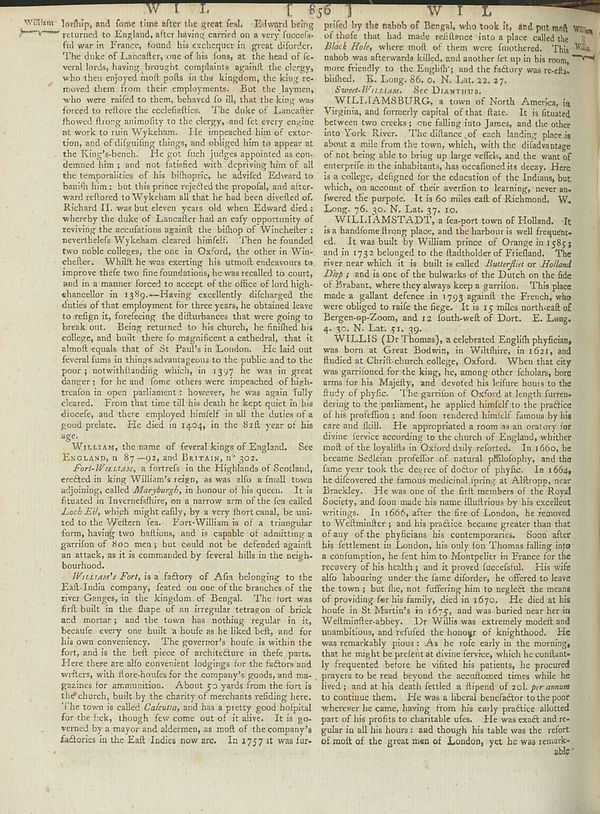
\includegraphics[width=0.85\textwidth]{../scans/page-0258-631a7ae7df34.jpg}
\caption*{Source scan: \texttt{page-0258-631a7ae7df34.jpg}}
\end{figure}

\end{document}
